\section{Small-Sample Confidence Intervals for $\mu$ and $\mu_1 - \mu_2$}

\nl So for for $\Xbar$ when $n$ is large, we have used
$$\frac{\that - \mu}{\sigma \big/ \sqrt{n}} \approx \frac{\that - \mu}{S \big/ \sqrt{n}}$$
\begin{center}{\color{red} for small $n$, no longer precise enough.}\end{center}

\nl But we set ourselves up for this issue back in Chapter 7.

\recall* We know $\displaystyle Z = \frac{\that - \mu}{\sigma \big/ \sqrt{n}}$ is distributed $N(0,\;1)$
\\and $\displaystyle V = \frac{(n-1)S^2}{\sigma^2}$ is distributed $\chi^2$ with $n-1$ df and $Z$ and $V$ are independent. Let
\begin{align*}
    T &= \frac{\Xbar - \mu}{S \big/ \sqrt{n}}\\
    &= \frac{\Xbar - \mu}{S \big/ \sqrt{n}} \cdot \over{s \big/ \sigma}\\
    &= \frac{\Xbar - \mu}{\sigma \big/ \sqrt{n}} \cdot \over{\sqrt{S^2 \big/ \sigma^2}}\\
    &= Z \cdot \frac{1}{\sqrt{\displaystyle\frac{(n-1)S^2}{\sigma^2} \bigg/ (n-1)}}
\end{align*}
We write $T = \dfrac{Z}{\sqrt{V \big/ r}}$ where $r = (n-1)$. \\\red{$T$ is the product of 2 pivotally distributed independent random variables.}

\defn We say $T$ has a $t$-sampling distribution ($t$-dist'n) with $(n-1)$ degrees of freedom and its pdf is given by
$$f_T(t) = \dfrac{\varGamma \pars{\dfrac{r+1}{2}}}{\sqrt{\pi r} \cdot \varGamma \pars{\dfrac{r}{2}}} \cdot \pars{1 + \dfrac{t^2}{r}}^{\textstyle-\frac{r+1}{2} }$$

\nl \textit{Remarks:}
\begin{enumerate}[label=\textcircled{\raisebox{-1pt}{\arabic*}}]
    \item We won't work with $f_T(t)$ explicity. \red{Note this distribution is pivotal... }  Independent of $\mu$ and $\sigma^2$. We pick our $t_{\alpha/2}$ from Table 5, page 849. Notice $\df = r = n-1 \geq 30$ are $Z$-scores:
    
    \nl To do so we need $\alpha$ and d.f. $= n-1$
    \newpage
    \addcontentsline{toc}{subsection}{Table 5: $t$-Distributions}
    \notab{\begin{center}
        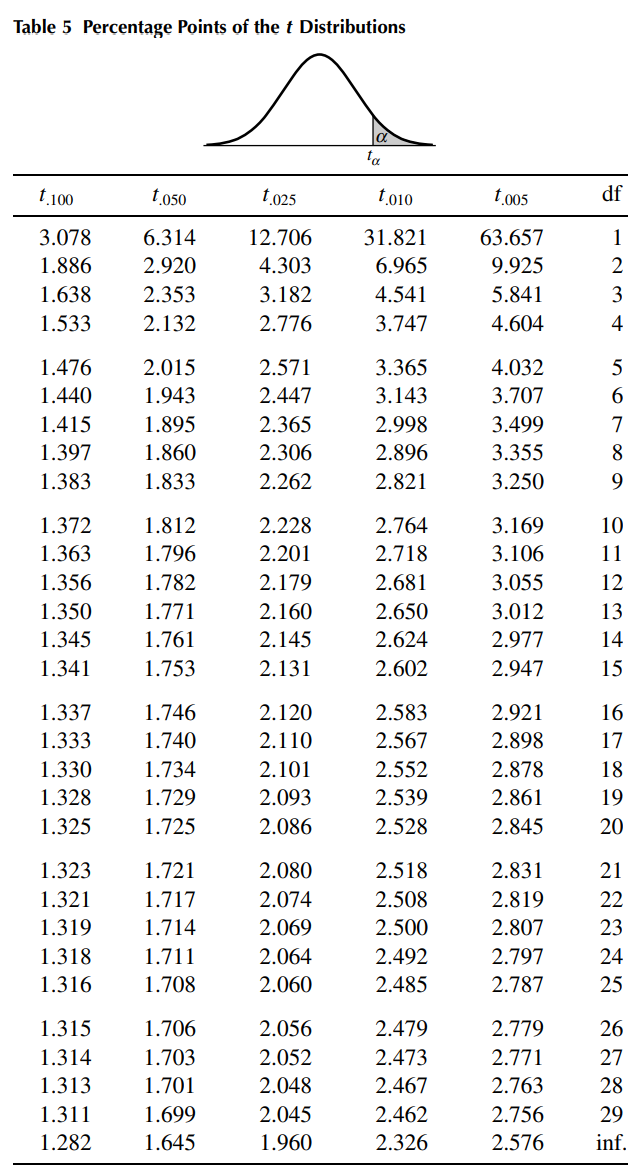
\includegraphics[width=5in]{Table5.png}
        \end{center}}
    \newpage
    \item $t$-distribution looks like \say{fat tailed} Normal Curves:
    \notab{\begin{center}
        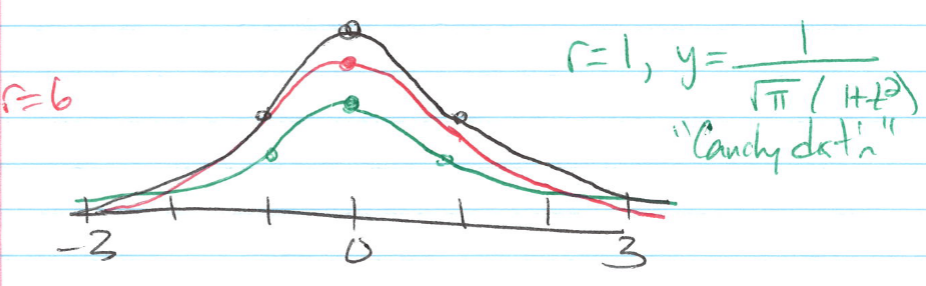
\includegraphics[width=5in]{8_8_rmk2.png}
        \end{center}}
    FACT: as $r \to \infty$, the D-distribution $\to N(0,\,1)$.

    \nl FUN FACT: Cauchy distribution is \say{famous}.
    $$r=1,\qquad \mu_T = 0, \quad \text{but} \quad \sigma^2_T = \infty$$

    \disc*    Small $n$ Confidence Interval.

    \nl For 2 sided, $T = \dfrac{\Xbar - \mu}{S \big/ \sqrt{n}}$
    \notab{\begin{center}
        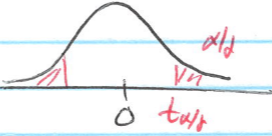
\includegraphics[width=2in]{8_8_im3.png}
        \end{center}}
    $$\P{-t_{\alpha/2} \, \leq \, T\, \leq t_{\alpha/2}} = 1 - \alpha$$
    $$\implies \Xbar \pm t_{\alpha/2} \pars{\dfrac{S}{\sqrt{n}}}$$

    \example $\quad n = 10, \qquad \Xbar = 3.22, \qquad S = 1.17$

    \nl Find a 95\% confidence interval for $\mu$.

    \nl Table 5: \hspace{.5cm} 95\% $\longrightarrow t_{0.025}$ with $\text{df} = (n-1) = 10-1 = 9$.

    \nl Use $t_{0.025} = 2.262$ and then $\Xbar \pm t_{0.025} \pars{\dfrac{S}{\sqrt{n}}} \implies 3.22 \pm (2.262) \pars{\dfrac{1.17}{\sqrt{10}}}$
    $$3.22 \pm 0.84 \; \implies \; (2.38,\;4.06)$$
    \newpage
    BONUS MATH: From the t-distribution.

    \nl For the math curious, it comes down to a fancy change of variables.

    \nl Recall from last semester, of $X$, $Y$ are independent, the joint pdf is $f(x,y) = f_x(x)f_y(y)$.

    \nl Here, $T = Z \pars{\dfrac{V}{r}}^{\textstyle  -\frac{1}{2} }$ and $Z$, $V$ are independent (as $\Xbar$ and $S$ are by Fisher's theorem).

    \nl To derive $f_T$, start with the join pdf of $Z$ and $Y$, a $\chi^2$ distribution of $r$ degrees of freedom. Then,
    $$f(y,z) = \frac{1}{\varGamma \pars{\dfrac{r}{2}} 2^{\scriptstyle r\scriptstyle/2 }} \cdot \displaystyle y^{\textstyle \frac{r}{2} \scriptstyle - 1} \cdot \exp\brac{-\frac{r}{2}} \cdot \over{\sqrt{2\pi}} \cdot \exp \brac{ \dfrac{Z^2}{2}} \qquad y\in(0,\;\infty), \quad Z \in \R$$
    Then let $t = Z \pars{\dfrac{V}{r}}^{\textstyle -\frac{1}{2}}, \qquad V = y$.
    \begin{align*}
        \P{Y<y,\; Z<z} &= \int_{-\infty}^{y} \int_{-\infty}^{z} f(y,z)\,dy\,dz\\
        &= \int_{-\infty}^{T} \int_{-\infty}^{V} f\Big(y(t,v),\, z(t,v)\Big) \red{\underbrace{\detx{Y_t}{Y_v}{Z_t}{Z_v}^{-1}}_{\text{Jacobian}}}  dt\,dv
    \end{align*}
    \setGreen Recall from MTH 420, for $u = h(x)$:
    $$\int_a^b f(x)\,dx = \int_{h(a)}^{h(b)} f\big(h^{-1}(a)\big) \frac{d}{dx}\Big(h^{-1}(u)\Big)\,du$$\setBlack

    \disc    Difference in means, small sample.

    \nl Start with $X,\; E[\,X\,] = \mu_x, \quad V[\,X\,] = \sigma^2_x$, \red{(Normal)}.\\
    And a r.v. $Y,\; E[\,Y\,] = \mu_y, \quad V[\,Y\,] = \sigma^2_y$, \red{(Normal)}.

    \nl Now we take 2 different iid random samples, which yields
    $$\Xbar \text{ and } S_{\Xbar}^2 \quad \text{with } \; n_1$$
    $$\Ybar \text{ and } S_{\Ybar}^2 \quad \text{with } \; n_2$$
    We have the unbiased estimator $\Xbar - \Ybar$ with $V(\Xbar - \Ybar) = \dfrac{\sigma^2_{\Xbar}}{n_1} + \dfrac{\sigma^2_{\Ybar}}{n_2}$. Then,
    $$Z = \frac{(\Xbar - \Ybar) - (\mu_x - \mu_y)}{\displaystyle \sqrt{\dfrac{\sigma^2_{\Xbar}}{n_1} + \dfrac{\sigma^2_{\Ybar}}{n_2}}} \quad \text{\red{a pivotal quantity.}}$$

    \nl Again, for small $n_i$, using $S_i \approx \sigma_i$ is not precise enough.

    \nl \red{Assumption: Let $\sigma_{\Xbar} = \sigma^{\Ybar}$. Thus}
    $$Z = \frac{(\Xbar - \Ybar) - (\mu_x - \mu_y)}{\displaystyle \sigma \sqrt{\dfrac{1}{n_1} + \dfrac{1}{n_2}}} \quad \text{\red{a pivotal quantity.}}$$

    \nl \red{Now we need to construct a point estimator for $\sigma$.}

    \nnl \textbf{Idea:} Try a \say{pooled} estimator.
    $$S_p^2 = \dfrac{\displaystyle \sum(X_i - \Xbar)^2 + \sum(Y_i-\Ybar)^2}{\red{r}}$$
    $$S_p^2 = \dfrac{\displaystyle (n_1-1) S_{\Xbar}^2 + (n_2-1) S_{\Ybar}^2}{\red{r}}$$
    Claim: $S_p^2$ is unbiased when $r = \big[ \red{(n_1-1)} + \red{(n_2-1)} \big] = n_1 + n_2 -2$. (i.e. $E[\,S^2_p\,] = \sigma^2 $)

    \nl \textit{Reason:} It is really the same computation as when we showed that $E[\,S^2\,] = \sigma^2$ when $S = \dfrac{1}{n-1}\displaystyle \sum(X_i-\Xbar)^2$\\Or, we can think about this as a product distribution of 2 independent $\chi^2$ distributions. One with $n_1-1$ df and another with $n_2-1$ df. Then (like with mgfs) the product distribution is $\chi^2$ with $n_1 - 1 + n_2 - 1$ df.

    \defn The \bu{pooled estimator} is
    $$S_p^2 = \dfrac{\displaystyle \sum(X_i - \Xbar)^2 + \sum(Y_i-\Ybar)^2}{n_1 + n_2 -2}.$$
    This is unbiased, and now we can define the t-statistic for $\mu_X - \mu_Y$ as
    $$T = \dfrac{(\Xbar-\Ybar)-(\mu_X-\mu_Y)}{S_p \displaystyle \sqrt{\dfrac{1}{n_1} + \dfrac{1}{n_2}}}.$$
    Which has $n_1 + n_2 - 2$ degrees of freedom.
\end{enumerate}